\chapter{Implementace}

\section{Implementace API}
Implementace původně probíhala ve frameworku FastAPI \sectionref{sec:api_technologies:fast}, ale po zjištění složitosti ORM při použití Python knihovny SQL Alchemy bylo doporučeno jedním z řešitelů (P. Mikula), použít raději Javu a její framework Spring Boot, za použití knihoven jako je JPA, Lombok, Jackson a jiných. Tato změna nebyla obtížná, jelikož vývoj byl teprve ve velice rané fázi vývoje. Taktéž Spring Boot byl jeden z kandidátů.

Nyní budou popsány nejdůležitější knihovny Frameworku Spring Boot, které byly použity při implementaci \gls{api}.


\subsection{Knihovny Spring Boot}\label{sec:impl:spring} 
% TODO nějaký lepší název nebo něco

Tyto knihovny jsou základním stavebním kamenem jak pro samotné koncové body tak pro \gls{orm}. Na obrázku \ref{fig:JPA} máme vizuální schéma toho, jak tyto knihovny spolu fungují.

\begin{figure}[ht!]
    \centering
    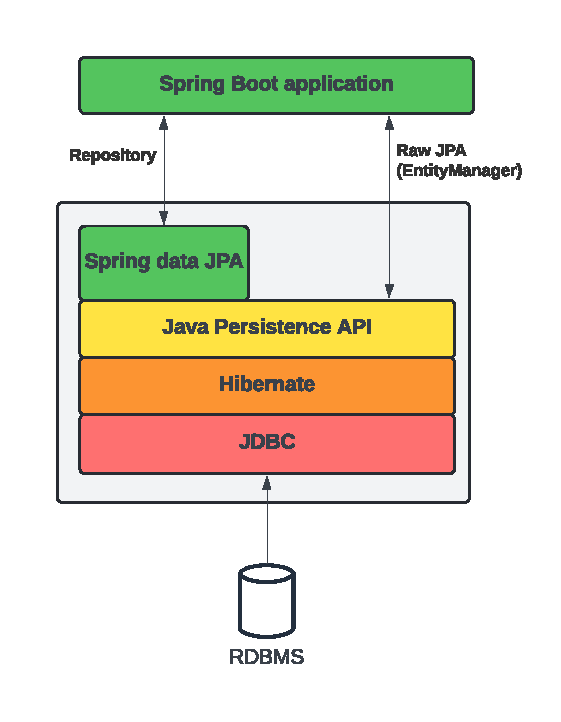
\includegraphics[width=0.5\textwidth]{figures/impl/API Implementation - JPA.pdf}
    \caption{Struktura Spring Boot Data JPA aplikace}
    \label{fig:JPA}
\end{figure}

\subsubsection*{Spring Data JPA}
JPA neboli Java Persistence API je jedna ze součástí Spring Data Family, která umožňuje jednoduché implementování \textbf{repozitářů} založených na JPA a signifikantně zjednodušuje implementaci datové vrstvy aplikace. Umožňuje používat základní SQL požadavky a ORM bez námahy vytvoření vlastních požadavků. V ukázce na výpisu \ref{code:JPA_repo} je vidět implementace repozitáře pro entitu \textit{Enemy}. Zde jsou již naimplementované základní metody jako \textit{save}, \textit{findAll}, a je zde navíc metoda \textit{findAllByLocationId} s vlastním SQL dotazem.

\begin{listing}[ht!]
    \inputminted[]{Java}{resources/code/impl/EnemyRepo.java}
    \caption{Ukázka JPA repozitáře}
    \label{code:JPA_repo}
\end{listing}

\subsubsection*{JPA}
Spring Data JPA používá několik dalších knihoven a dalo by se říci, že to je jakýsi zprostředkovatel nad \textbf{JPA}. JPA zajišťuje objektově relační mapování (\gls{orm}), což usnadňuje práci s ukládáním objektů do databáze a naopak.

Základním objektem v JPA je \textit{Entita}. Ta reprezentuje objekt v databázi, který je poté namapován na jednotlivé vlastnosti třídy \coderef{code:jpa_entity}. Třídu označíme jako entitu pomocí anotace \textit{@Entity} a poté pomocí \texttt{@Table} můžeme upřesnit jméno tabulky, schéma databáze a jiné atributy. Za pomoci anotace \textit{@Id} označíme primární klíč a nebo pomocí \texttt{@EmbeddedId} označíme složený primární klíč. Atributy třídy označíme pomocí \texttt{@Column} kdy ve výchozím stavu atribut může nabývat prázdné hodnoty a sloupec v databázi se jmenuje stejně jako atribut. Relace se mapují pomocí jedné z anotací \texttt{@OneToOne}, \texttt{@OneToMany}, \texttt{@ManyToOne} nebo \texttt{@ManyToMany} podle toho, jakou relaci potřebujeme. V této implementaci probíhal nejdříve návrh databáze, takže jsme používali pouze \texttt{1:N} relace abychom se vyhnuli cyklickým závislostem, protože vazební \texttt{M:N} tabulky již byly v databázi.

\subsubsection*{Hibernate}\label{sec:impl:hibernate}
Jedna z konkrétních implementací JPA je Hibernate. Za pomocí výše zmíněných anotací nebo XML \sectionref{sec:formats:xml} schématu si udržuje schéma databáze a stav objektů, udržuje tedy data perzistentní. Díky schématu databáze Hibernate ví, jak se mají data z databázových tabulek transformovat do objektů a naopak. \cite[]{enwiki:1217225259}

\subsubsection*{JDBC}\label{sec:impl:jdbc}
Neboli Java Database Connectivity je API pro přístup k databázi. Poskytuje metody pro dotazování se na na databázi pomocí \gls{sql} a umožňuje zpracovávat výsledky dotazů.

\begin{listing}[ht!]
    \inputminted[breaklines]{Java}{resources/code/impl/EnemyDTO.java}
    \caption{Příklad entity v JPA}
    \label{code:jpa_entity}
\end{listing}


\subsection{Jiné použité knihovny} %%TODO reformat nadpis aaaaaa
V této kapitole budou popsány knihovny, které nejsou součástí Spring Bootu, ale byly ve větší míře použity při implementaci API.

\subsubsection*{Lombok}\label{sec:impl:lombok}
Lombok je knihovna, která za pomocí anotací automaticky generuje základní repetetivní kódy jako jsou gettery a settery, konstruktory a jiné, což je pro vývojáře velice vítané.

První možností této knihovny jsou anotace \texttt{@Getter} a \texttt{@Setter}, které automaticky vygenerují \textbf{gettery} nebo \textbf{settery} s příslušnými modifikátory přístupu pro daný atribut \coderef{code:lombok:getters}. Tato anotace lze použít i nad celou třídou a automaticky vygeneruje kód pro všechny atributy. Vygenerované metody jsou ukázány na výpisu \ref{code:lombok:getters:generated}.

\begin{listing}[H]
    \begin{minted}[fontsize=\footnotesize]{Java}
        public class GetterSetterExample {
            @Getter private int age = 10;
            @Setter(AccessLevel.PROTECTED) private String name;
        }
     \end{minted}
    \caption{Použití anotací \texttt{@Getter} a \texttt{@Setter}}
    \label{code:lombok:getters}
\end{listing}

\begin{listing}[H]
    \begin{minted}[fontsize=\footnotesize]{Java}
        public class GetterSetterExample {
            private int age = 10;
            private String name;
            public int getAge() {
                return this.age;
            }
            protected void setName(String name) {
                this.name = name;
            }
        }
     \end{minted}
    \caption{vygenerovaný kód za pomocí \texttt{@Getter} a \texttt{@Setter}}
    \label{code:lombok:getters:generated}
\end{listing}

Další důležité anotace se týkají konstruktorů. \texttt{@NoArgsConstructor} vygeneruje prázdný konstruktor, \texttt{@AllArgsConstructor} vygeneruje konstruktor se všemi atributy \coderef{code:lombok:constructor} a jako poslední anotace \texttt{@RequiredArgsConstructor} vygeneruje konstruktor s všemi atributy označenými jako \texttt{@NonNull}. Tato anotace se zapisuje nad třídu. \cite{lombok:constructor} 

\begin{listing}[H]
    \begin{minted}[fontsize=\footnotesize]{Java}

        public class ConstrExample {
            private int age;
            private String name;

            ConstrExample(int age, String name) {
                this.age = age;
                this.name = name;
            }
        }
    
    \end{minted}
    \caption{Příklad kódu vygenerovaného pomocí \texttt{@AllArgsConstructor}}
    \label{code:lombok:constructor}
\end{listing}


Práci si je možné zjednodušit ještě více za pomocí anotace \texttt{@Data}, která vygeneruje výše zmíněné \texttt{@Getter, @Setter, @RequiredArgsConstructor} a navíc \texttt{@ToString} a \texttt{@EqualsAndHashCode}.\cite{lombok:data} Anotace \texttt{@ToString} vygeneruje metodu \texttt{toString()}, která objekt převede na textový řetězec, kde za pomoci různých parametrů můžeme upravovat, které atributy se budou vypisovat a jak. Další anotace, kterou \texttt{@Data} obsahuje, je \texttt{@EqualsAndHashCode}, která vygeneruje metody pro porovnávání objektů.

Za zmínku také stojí anotace \texttt{@Builder}, která vygeneruje interní třídu podle návrhového vzoru Builder\cite{refactoringGuru:builder}, jež slouží k vytváření objektů. \cite{lombok:builder}

\subsubsection*{Jackson}\label{sec:impl:jackson}
Tato knihovna slouží pro serializaci objektů do formátu JSON \chapterref{sec:formats:json} a naopak. S její pomocí bylo možné specifikovat, jak se budou jednotlivé objekty či atributy serializovat, například zde lze nastavit ignorování některých atributů nebo úplně vlastní serializace.

\subsubsection*{Swagger}\label{sec:impl:swagger}
Swagger je open-source dokumentační nástroj pro \gls{restful api} zahnutý přímo v knihovně Spring Boot, který umožňuje vývoj API skrz celý jeho životní cyklus od návrhu přes dokumentaci a testování po nasazení. Využívá specifikaci OpenAPI, pomocí které dokáže generovat dokumentaci, interakci, testy a další.\cite{swagger:about} Tohoto nástroje jsme hojně využívali zvlášť pro interakci s koncovými body pro testování.

Ve Spring Bootu je jeho použití velmi jednoduché, stačí zaznamenat závislosti do \texttt{pom.xml} a přidat Springdoc Swagger konfiguraci do hlavního konfiguračního souboru.

\subsection{Serializace}\label{sec:impl:serialization} 
% todo oprav si tu vetu pls wtf is this
% V rámci vývoje byla vytvořena vlastní třída pro serializaci relačních objektů pomocí vlastní třídy 
% %\coderef{code:lazyFieldsSerializer} TODO odkaz v přiložených souborech jaký to je soubor JEBAT THIS SHIT
% na serializování mapovaných objektů. 
Pro serializaci \sectionref{sec:formats:deserialization} relačních objektů byla vytvořena třída \texttt{LazyFieldsSerializer}, která se stará o serializaci objektů, které jsou označeny jako \texttt{lazy}.
Upravená metoda \texttt{serialize} zde zkontroluje, zda je serializovaný objekt instancí proxy a pokud ano, zda je objekt nainicializován. To za nás řeší metoda \texttt{Hibernate.isInitialized}. 
%\coderef{code:lazyFieldsSerializer}[, řádek 56]. TODO to stejné jako výše
Pokud je tedy objekt nainicializován, serializuje se a dále na se jeho atributech opět volá metoda \texttt{serialize}. Pokud není nainicializován a nejedná se o kolekci, tak se serializuje pouze jeho id aniž by se objekt nainicializoval celý.
%\coderef{code:lazyFieldsSerializer}[, řádek 60]. TODO to stejné jako výše
Pokud se jedná o kolekci, musí se jednat o \texttt{M:N} tabulku a serializují se tedy všechny atributy kromě relací. 
%\coderef{code:lazyFieldsSerializer}[, funkce \texttt{writeFieldsWithoutLazy() }]. TODO to stejné jako výše 


\subsection{Lazy load}\label{sec:impl:lazyload}
Pro tento účel musela být vytvořena metoda pro postupnou inicializaci. Pro rekurzivní načítání relačních objektů byla vytvořena statická metoda \texttt{hibernateInitializeAll()}, která přijme objekt a rekurzivně načte všechny jeho relace.
% nějaký ref
Tato funkce za pomocí \texttt{Hibernate.initialize()} nejdříve nainicializuje vstupní objekt a poté rekurzivně prochází všechny jeho atributy, přičemž přeskakuje ty, které nemají jednu z relačních anotací. Funkce má taktéž podporu filtru pro samotný lazy load, když se jméno atributu shoduje s jakýmkoli slovem ve filtru, atribut se přeskočí v inicializování.


\subsection{Koncové body}\label{sec:impl:endpoints}
Hlavním výstupem této práce je seznam koncových bodů \figureref{fig:action:endpoint} , které je možné použít pro administrativní část i hraní hry. Jednotlivé přístupové body jsou rozděleny do tzv. kontrolérů. Jako příklad zde je kontrolér pro entitu \textit{Character} \coderef{code:characterController}. 

Níže \figureref{fig:endpoint:general} je zobrazen obecný diagram komponent koncového bodu. Třída \texttt{Controller} zde představuje komponentu poskytující koncové body klientům. Po příchozím požadavku ho přeposílá třídě \texttt{Service}, která se stará o jeho vyhodnocení. Při kladném výsledku data předá zpět třídě \texttt{Controller}, která je výsledek pošle klientovi. Pokud je výsledek záporný, je zachycena výjimka a klientovi je vracena přímo.

\begin{figure}[ht!]
    \centering
    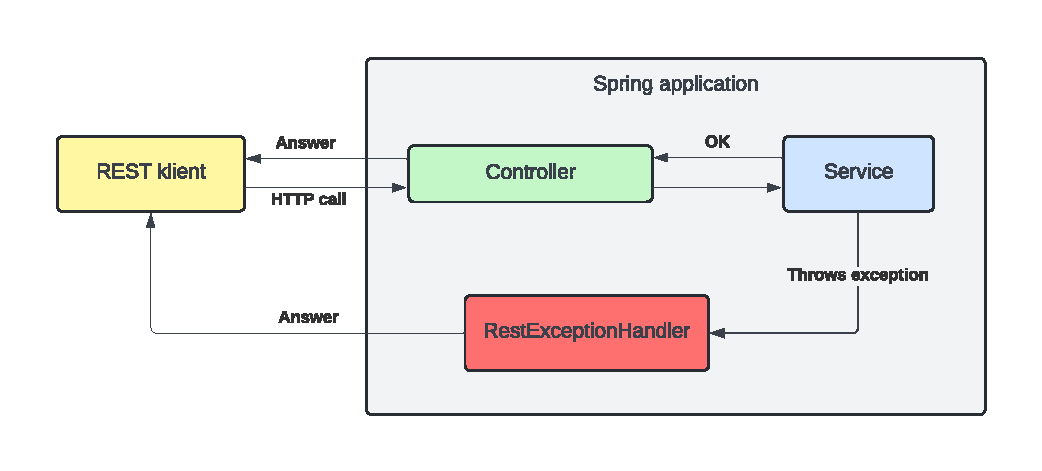
\includegraphics[width=0.9\textwidth]{figures/impl/API Implementation - endpoint.pdf}
    \caption{Obecný diagram koncového bodu}
    \label{fig:endpoint:general}
\end{figure}

Anotací \texttt{@RestController} určíme, že tato třída bude obsahovat koncové body. Dále pomocí anotace \texttt{@RequestMapping} zadáme cestu, pod kterou budou všechny koncové body v této třídě dostupné. A na závěr pomocí jednotlivých mapping anotací (\texttt{@GetMapping, @PutMapping @PostMapping @DeleteMapping}) určujeme, na jakou HTTP metodu má funkce reagovat.

Při mapování můžeme používat jak URI vzory pomocí regex výrazů (např \texttt{"/resources/*.png"}) tak i proměnné v URI (např \texttt{"/resources/{id}"}). Ten používáme třeba zde na výše zmíněném výpisu kontroléru postavy \coderef{code:characterController}[, řádek 9] pro získání jedné entity \textit{Character}. S tím se pojí anotace \texttt{@PathVariable}, která určuje, že vstupní parametr id bude brán z URI a bude se jednat o datový typ \texttt{int}.

Jako další můžeme používat tzv. \textit{query} parametry, které je možné získat získat za pomocí anotace \texttt{@RequestParam}, kde se může předem určit, zda je parametr povinný nebo jakou bude mít výchozí hodnotu \coderef{code:characterController}[, řádek 12]. Ve výsledné URI požadavek pro získání entity s identifikátorem 1 a načteným inventářem bude vypadat následovně: \texttt{GET /characters/1?include=inventory\&} \texttt{lazy=true}. Tento požadavek vrátí postavu hráče s namapovaným inventářem a s ostatními atributy. Atributy \textit{clazz} a \textit{race} \figureref{fig:dix:database_schema}
budou vypsané pouze jako id a nebudou nainicializované.

Pro metody post byla ještě použita anotace \texttt{@RequestBody}, pomocí které můžeme vzít data z těla požadavku. V našem případě jsme požadovali JSON objekt, který se hned mapoval na objekt třídy.

\begin{listing}[ht!]
    \inputminted[]{Java}{resources/code/impl/CharacterController.java}
    \caption{Kontrolér pro entitu \textit{Character}}
    \label{code:characterController}
\end{listing}


\section{Testování}\label{sec:testing}
Testování probíhalo za pomocí dobrovolníků kteří si zkusili zahrát hru, nebo díky dokumentačnímu rozhraní Swagger \sectionref{sec:impl:swagger} pohodlně testovali přímo koncové body v API.



\section{Problémy při vývoji}\label{sec:impl:problems}
Během vývoje se vyskytlo několik problémů, které se musely vyřešit. Nyní se zaměříme na ty nejzávažnější.

\subsection{Serializace}
Když byly atributy označeny jako \texttt{lazy}, pořád byl problém při serializaci, kdy k těmto atributům knihovna Jackson přistupovala, čímž byly načteny z databáze a následně serializovány, i když se v kódu s nimi nepracovalo. Tento problém byl vyřešen pomocí vlastní třídy \texttt{LazyFieldsSerializer}
na serializování namapovaných objektů. \sectionref{sec:impl:serialization}

\subsection{Lazy load}
Knihovna Hibernate bohužel nemá metodu pro rekurzivní načtení relací objektu, v souvislosti s vlastní serializací pak nastal problém, když se měl serializovat objekt se všemi jeho relacemi. Hibernate podporuje jen načtení objektu který je instancí \texttt{HibernateProxy}. Tento problém byl vyřešen pomocí statické funkce \texttt{hibernateInitializeAll()}. \sectionref{sec:impl:lazyload}

\subsection{Příliš velká databáze}
Při návrhu databáze nebyl brán ohled na možnou časovou náročnost. Databáze se navrhovala jako funkční celek připravený do produkce s ohledem na případné rozšíření. To vyústilo v problém, kdy jednotlivé případné úkony jako je \gls{orm} či CRUD operace nad jednotlivými entitami byly velice zdlouhavé a zabíraly většinu času vývoje. S tímto se pojil o to složitější management změn u koncových bodů. Z tohoto důvodu se v implementaci vynechaly entity \textit{summon} a \textit{item}.
